\section{Meta-Análise, Resumo e Referências}

\begin{frame}{Meta-Análise: Uma Visão Cética e Saudável}
    \begin{block}{O Limite da Amostra Pequena}
        Nossos resultados provam causalidade para os $31$ pacientes específicos que participaram do estudo. Mas e para a população geral de pacientes?
    \end{block}
    \begin{block}{A Meta-Análise de 2011}
        Pesquisadores reuniram todos os estudos mundiais de Toxina Botulínica para dor lombar crônica.
        \begin{itemize}
            \item $19$ estudos foram excluídos devido à falta de randomização ou dados incompletos.
            \item Apenas $3$ estudos controlados aleatórios restaram (incluindo o que analisamos).
            \item \textbf{Conclusão:} As evidências clínicas acumuladas ainda são classificadas como de \textbf{baixa qualidade}. Mais pesquisas com amostras maiores são fundamentais antes de uma recomendação de larga escala.
        \end{itemize}
    \end{block}
\end{frame}

\begin{frame}{O Trabalho do Cientista de Dados}
    \begin{block}{O Rigor da Ciência de Dados}
        Qualquer ciência (inclusive a nova ``ciência de dados'') é um caminho complexo que exige rigor analítico e ética na interpretação.
    \end{block}
    \begin{block}{Nosso Repertório de Ferramentas}
        \begin{itemize}
            \item Até o momento, aprendemos apenas uma ferramenta básica: testes de hipóteses via permutação e bootstrap.
            \item Existem limitações claras nos testes clássicos, mas se bem interpretados, oferecem bases sólidas de decisão.
            \item \textbf{Próximos Passos (Olhando para o Futuro):} Após a avaliação, expandiremos nossas capacidades com modelos preditivos:
            \begin{itemize}
                \item \textbf{Regressão:} Previsão de valores contínuos.
                \item \textbf{Classificação:} Atribuição de rótulos categóricos.
            \end{itemize}
        \end{itemize}
    \end{block}
    \centering
    \textit{Lembre-se: não seja o profissional de uma ferramenta só!}
\end{frame}

\begin{frame}{O Caso da Cloroquina: O Perigo da Falta de Randomização}
    \begin{columns}
        \begin{column}{0.55\textwidth}
            \begin{block}{O Erro de Randomização}
                Os autores do famoso estudo sobre cloroquina e azitromicina admitiram: \textbf{o estudo não foi randomizado}.
            \end{block}
            \begin{itemize}
                \item \textbf{Falta de Sorteio:} Os pacientes escolheram se tomavam ou não a medicação, gerando um grave viés de seleção.
                \item \textbf{Consequência:} Sem randomização, premissas de causalidade caem por terra.
                \item \textbf{Consenso Posterior:} Estudos subsequentes robustos confirmaram a ineficácia do tratamento.
            \end{itemize}
        \end{column}
        \begin{column}{0.45\textwidth}
            \centering
            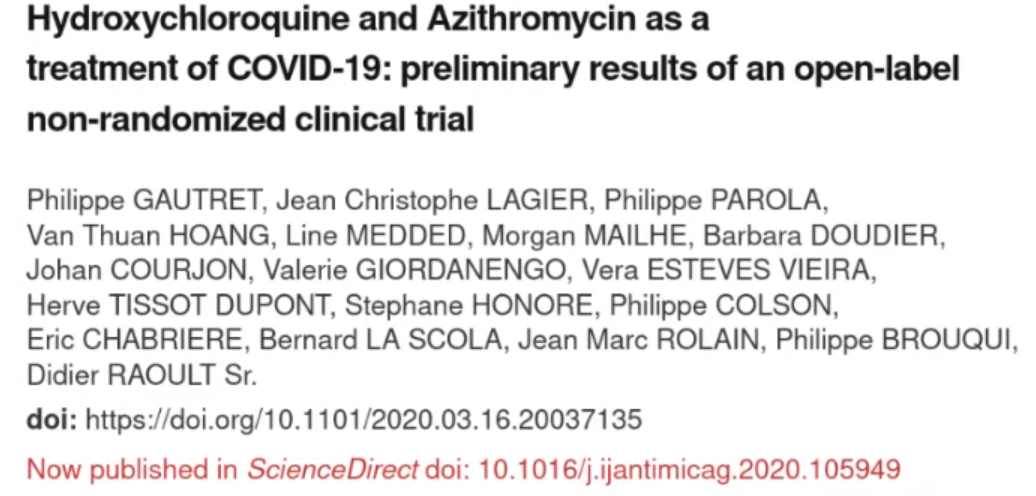
\includegraphics[width=\textwidth]{estudo_cloroquina.png}
            \vspace{0.1cm}
            \tiny{Título do artigo demonstrando a natureza não-randomizada (\textit{open-label non-randomized}).}
        \end{column}
    \end{columns}
\end{frame}

\begin{frame}{Método Científico}
    \begin{itemize}
        \item O arcabouço de testes de hipóteses é uma ótima ferramenta para a ciência no geral.
        \item Afinal, testar hipóteses é o grande objetivo da ciência!
        \item Note que nem toda Ciência vai usar Estatística ou Ciência de Dados.
        \item Existem várias formas de fazer experimentos/métodos:
        \begin{itemize}
            \item \textbf{Experimentos Físicos:} Equações para explicar o nosso mundo comprovadas via experimentos.
            \item \textbf{Qualitativos:} Estudos onde não necessariamente usamos dados ou médias, mas que ainda assim são feitos com \textbf{método}.
            \item \textbf{Tentativas de Provas para os Teóricos:} Cada tentativa de prova matemática é uma hipótese, por exemplo.
        \end{itemize}
    \end{itemize}
\end{frame}

\begin{frame}{Ciência de Dados no mundo da Ciência}
    \begin{block}{A Incerteza nos Dados}
        ``All datasets involve uncertainty. There may be uncertainty about how they were collected, how they were measured, or the process that created them. Statistical modeling helps quantify and reason about uncertainties in a systematic way.''
    \end{block}
    \begin{alertblock}{Conclusão Importante}
        A Ciência de Dados \textbf{não é toda a ciência}! Ela apenas \textbf{ajuda no método científico} ao fornecer uma forma sistemática de analisar dados e quantificar incertezas.
    \end{alertblock}
\end{frame}

\begin{frame}{O Ciclo do Método Científico}
    O avanço da ciência baseia-se em um ciclo sistemático e replicável:
    \begin{block}{As Fases do Ciclo:}
        \begin{enumerate}
            \item \textbf{Pergunta:} Formulada de maneira clara (ex: Fumar na gestação afeta o peso do recém-nascido?).
            \item \textbf{Revisão de Literatura:} Investigar o que a comunidade científica já descobriu sobre o assunto.
            \item \textbf{Hipótese:} Definir o modelo nulo ($H_0$) e a alternativa de efeito ($H_1$).
            \item \textbf{Experimento:} Testes A/B aleatórios são fundamentais para gerar dados confiáveis.
            \item \textbf{Análise do Resultado:} Avaliação da significância e do tamanho do efeito.
            \item \textbf{Comunicação:} Publicar os resultados com os métodos claros para permitir a replicação.
        \end{enumerate}
    \end{block}
\end{frame}

\begin{frame}{A Replicação como Regra de Ouro}
    \begin{block}{Se não é replicável, não é ciência!}
        \begin{itemize}
            \item Um único experimento com resultado positivo (como BTA para dor lombar com $N=31$) não é definitivo.
            \item Existe sempre uma chance de erro estatístico ou viés na amostra local.
            \item Um novo experimento, sob as mesmas hipóteses e feito por outro pesquisador, deve ser capaz de reproduzir o efeito.
        \end{itemize}
    \end{block}
    \begin{block}{Meta-Análise}
        O estudo que consolida os resultados de múltiplos experimentos independentes. É a meta-análise que estabelece o consenso científico final sobre a eficácia de um tratamento.
    \end{block}
\end{frame}

\begin{frame}{Críticas aos Testes de Hipóteses e P-valores}
    \begin{block}{A Crítica ao Limiar dos 5\%}
        Há um movimento de estatísticos e cientistas contra o uso mecânico e cego da regra de significância de $p < 0.05$.
        \begin{itemize}
            \item Críticos apontam problemas de ``P-hacking'' (manipulação de dados até obter P-valor significativo) e o viés de publicação.
            \item Um P-valor sozinho não mede a força da evidência ou a importância prática de um resultado.
        \end{itemize}
    \end{block}
    \begin{alertblock}{O que relatar em seus estudos?}
        Para garantir o rigor, sempre apresente: (1) O valor exato do P-valor, (2) O tamanho amostral ($N$), (3) O tamanho do efeito (effect size) e (4) Como testou (ex: Bootstrap vs. Permutação).
    \end{alertblock}
\end{frame}

\begin{frame}{Resumo e Principais Aprendizados}
    \begin{block}{Ideias Fundamentais da Aula}
        \begin{itemize}
            \item \textbf{Causalidade vs. Associação:} Experimentos Controlados Aleatórios (RCTs) neutralizam fatores de confundimento, permitindo comprovar causa e efeito.
            \item \textbf{Resultados Potenciais:} A conceituação imaginária de todos os cenários possíveis para cada indivíduo (metáfora do bilhete).
            \item \textbf{Teste de Permutação:} O embaralhamento computacional de rótulos simula o acaso sob a hipótese nula $H_0$.
            \item \textbf{P-valor Empírico:} Permite determinar se a diferença observada é comum ou extremamente improvável sob o acaso.
            \item \textbf{Método Científico:} Rigor, replicação e pensamento crítico são fundamentais na análise de dados.
        \end{itemize}
    \end{block}
\end{frame}

\begin{frame}{Referências Bibliográficas}
    \begin{block}{Leituras Recomendadas}
        \footnotesize
        \begin{itemize}
            \item \textbf{Learning Data Science} \\
            Sam Lau, Joey Gonzalez, and Deb Nolan. \\
            Capítulo 17: Inference, Prediction, and Generalization. \\
            \url{https://learningds.org/ch/17/inf_pred_gen_HT.html}
            \vspace{0.3cm}
            \item \textbf{Computational and Inferential Thinking} \\
            Ani Adhikari and John DeNero. \\
            Capítulo 11: Testing Hypotheses (Seção 11.1 - Causality). \\
            \url{https://inferentialthinking.com/chapters/11/testing-hypotheses/}
        \end{itemize}
    \end{block}
\end{frame}
